\section{REFERENCIAL TEÓRICO}
Neste tópico, apresenta-se o referencial teórico que fundamenta esta pesquisa. Conceituam-se as principais teorias que serviram de fundação para o \textit{game design} e elementos do game design, definição do gênero e de jogos sérios.

\subsection{Teoria da Autodeterminação (SDT) e motivação}
Proposta por Richard Ryan e Edward Deci \cite{Ryan1985}, a Teoria da Autodeterminação (SDT) é uma estrutura organísmica \cite{Ryan2020} que assume que os seres humanos possuem uma propensão inerente para o crescimento e a integração, mas necessitam de suportes ambientais para florescer \cite{Ryan1985}. A teoria postula três necessidades psicológicas fundamentais e universais \cite{Ryan1985}: a autonomia, que compreende o senso de iniciativa e propriedade sobre as ações; a competência, referente ao sentimento de maestria e eficácia; e o relacionamento, que abrange o senso de pertencimento e conexão social \cite{Shi2016}. Como essas necessidades se relacionam com a motivação, pode ser visto na Fig. \ref{fig:sdt}.

\begin{figure}[H]
    \centering
    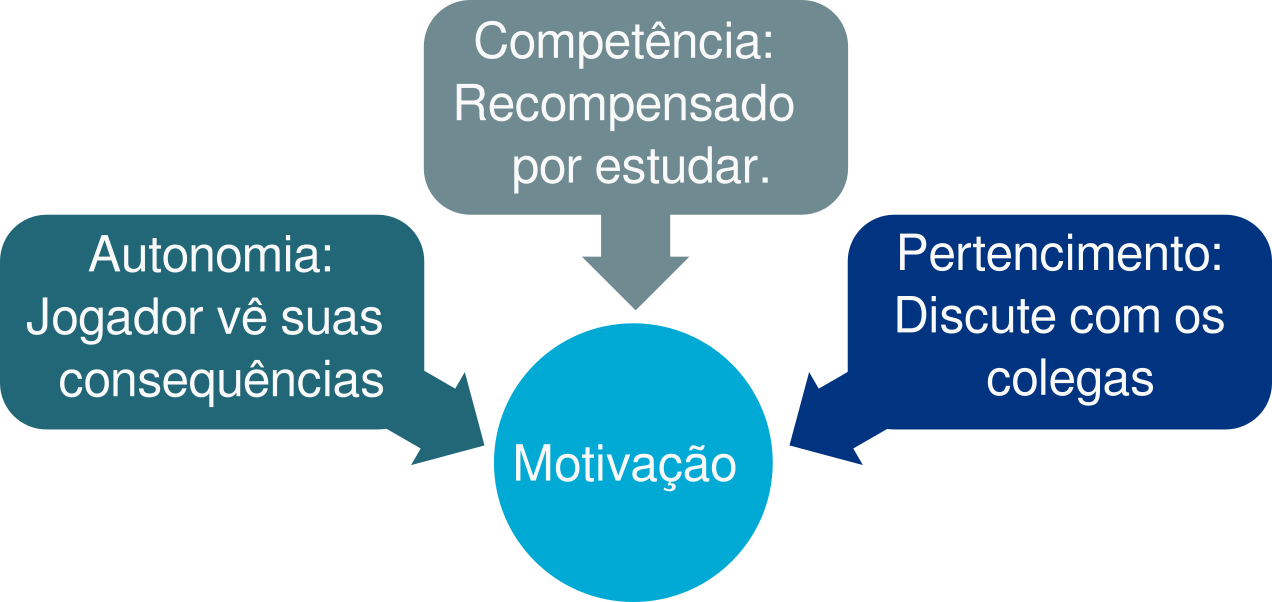
\includegraphics[width=0.4\textwidth]{images/sdt.png}
    \caption{Teoria da Autodeterminação (SDT). Fonte: elaborado pelo autor.}
    \label{fig:sdt}
\end{figure}

Ryan e Deci \cite{Ryan1985} dividem a motivação em dois tipos principais: motivação intrínseca, que é impulsionada por interesses e prazeres inerentes à atividade, e motivação extrínseca, orientada por recompensas ou pressões externas. Nos jogos, a motivação intrínseca é desenvolvida quando o design proporciona ao jogador agência para completar objetivos, além de permitir novas tentativas após falhas (\textit{graceful failure}) e a colaboração com outros jogadores \cite{Plass2020}. A motivação extrínseca, por sua vez, é frequentemente implementada por meio de sistemas de recompensas, como pontos, medalhas e tabelas de classificação \cite{Coelho2025}.

Ao aprofundar a análise da SDT no contexto lúdico, a Teoria da Integração Organísmica (OIT) \cite{Ryan2022} explica como comportamentos inicialmente motivados por fatores externos podem ser internalizados e integrados ao \textit{self}. Para que essa transição ocorra, o ambiente de jogo deve possuir uma significância funcional informacional \cite{Gao2024}, na qual o jogador percebe o \textit{feedback} e as recompensas como suportes à sua competência, e não como mecanismos de controle. 

Estudos indicam que o uso de recompensas pode minar a motivação intrínseca se forem compreendidas como controladoras, por reduzir a autonomia do jogador \cite{Ryan2022}. Inversamente, recompensas intrínsecas, que oferecem novas habilidades ou acesso a conteúdos, reforçam o engajamento volitivo \cite{Ryan2022}, definido como o estado de envolvimento ativo e focado no jogo. Além disso, a satisfação das necessidades é mutuamente informativa, pois a competência só gera motivação de alta qualidade quando acompanhada por um senso de autonomia, permitindo que o jogador sinta-se o \textit{locus} de causalidade de seu sucesso \cite{Ryan1985, Gao2024}.

\subsection{Teoria da Aprendizagem Significativa (TAS) e organizadores prévios}
David Ausubel fundamentou a Aprendizagem Significativa (TAS) \cite{Ausubel1963} no princípio de que novas ideias são assimiladas apenas quando ancoradas em conhecimentos prévios estáveis, processo denominado subsunção \cite{Espirito2020}. Para mitigar o distanciamento entre o que o estudante já sabe e o material novo, Ausubel \cite{Ausubel1963} propôs o uso de organizadores prévios, que são materiais introdutórios apresentados em um nível mais alto de abstração e generalidade. Esses materiais servem como pontes conceituais para destacar a importância do novo conteúdo \cite{Custodio2015}. No \textit{design} de jogos, isso se manifesta em tutoriais que apresentam a estrutura do sistema antes da complexidade total, permitindo a diferenciação progressiva do conhecimento \cite{Espirito2020, Custodio2015}.

Recentes revisões críticas da TAS, fundamentadas em avanços da neurociência, sugerem que a memória não é um constructo estático, mas um processo dinâmico e generativo \cite{Bryce2024}. Sob esta ótica, a aprendizagem significativa não envolve a substituição de concepções intuitivas, conhecidas como alternativas, mas sim um processo de coexistência conceitual e revisão. Nesse processo, o aprendiz desenvolve a habilidade de selecionar o repertório (\textit{scaffolding}), seja ele cotidiano ou científico, mais adequado à situação imediata. Em vez de apenas suportes temporários (\textit{scaffolding}), propõe-se o uso de \textit{cantilevers} conceituais , que são estruturas de apoio permanentes baseadas no conhecimento prévio que sustentam a construção de novos saberes \cite{Bryce2024}. Tal analogia pode ser compreendiada na Fig. \ref{fig:tas}.

\begin{figure}[H]
    \centering
    
\includegraphics[width=0.4\textwidth]{images/tas.png}
    \caption{Teoria da Aprendizagem Significativa (TAS). Fonte: elaborado pelo autor.}
    \label{fig:tas}
\end{figure}

\subsection{Aprendizagem Tangencial}
A Aprendizagem Tangencial \cite{Portnow2012} refere-se ao processo espontâneo no qual o jogador adquire conhecimentos periféricos ao interagir com mídias de entretenimento que não têm o ensino como objetivo primário \cite{Mozelius2017}. Isso ocorre quando o jogador se envolve com elementos ludo-narrativos \cite{LimadaCostaJunior2022}, a exemplo da história de \textit{Assassin's Creed} ou das mecânicas de química em Batalha Quimicard \cite{GomesdeFreitas2017}, e busca voluntariamente aprofundar esses temas em fontes externas \cite{Lorenzatti2020}. Tal interação pode ser visualizada na Fig. \ref{fig:tangencial}. Designers utilizam ferramentas referenciais como enciclopédias \textit{in-game}, espaços informativos em telas de carregamento com curiosidades e referências diretas a artefatos reais para estimular essa curiosidade \cite{Lorenzatti2020}.

\begin{figure}[H]
    \centering
    
\includegraphics[width=0.4\textwidth]{images/tangencial.png}
    \caption{Aprendizagem Tangencial. Fonte: elaborado pelo autor.}
    \label{fig:tangencial}
\end{figure}

A eficácia desse processo pedagógico está intimamente ligada à integração intrínseca do conteúdo às mecânicas de vitória, a fim de que o objeto de conhecimento constitua a própria natureza do jogo e não um elemento meramente ilustrativo ou uma barreira enfadonha \cite{Mozelius2017}. Estudos indicam que, em jogos nos quais o conhecimento foi integrado com sucesso, as mecânicas servem como plataformas experimentais para que o jogador teste conceitos adquiridos externamente \cite{Mozelius2017}. No jogo sério Batalha Quimicard \cite{GomesdeFreitas2017}, por exemplo, a internalização de constantes como $K_a$ e $K_b$ para formular estratégias de duelo demonstra como o jogador se apropria do conceito científico para obter êxito sistêmico.

\subsection{Taxonomia de Bloom}
A Taxonomia de Bloom \cite{Bloom1956}, sistematizada em 1956 e revisada por Anderson e Krathwohl em 2001 \cite{Anderson2001}, categoriza os processos cognitivos em níveis de complexidade crescente: Lembrar, Compreender, Aplicar, Analisar, Avaliar e Criar. Pode ser compreendida como uma pirâmide, a exemplo da Fig. \ref{fig:bloom}, que inicia com os níveis baixos de Lembrar e Compreender. No design de jogos sérios \cite{Plass2020}, esse \textit{framework} é utilizado para alinhar a mecânica de jogo ao desempenho acadêmico esperado, garantindo que o conteúdo seja introduzido de forma estruturada.

\begin{figure}[H]
    \centering
    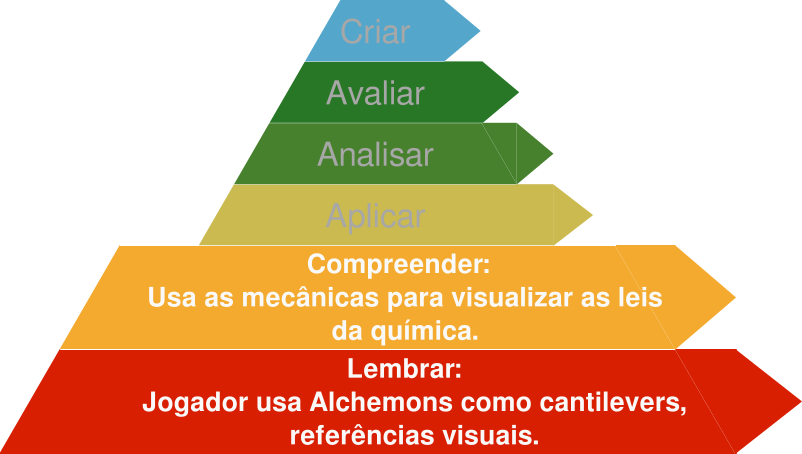
\includegraphics[width=0.4\textwidth]{images/bloom.png}
    \caption{Taxonomia de Bloom. Fonte: elaborado pelo autor.}
    \label{fig:bloom}
\end{figure}

Diferente de abordagens que buscam a maestria total do espectro cognitivo, o Alchemon foca deliberadamente nos níveis de ordem inferior: Lembrar e Entender \cite{KrishnaShinde2025}. O objetivo central é a consolidação de conhecimentos factuais e conceituais, como o reconhecimento de símbolos químicos e a compreensão de fenômenos básicos \cite{Tuomisto2015}. Assim, servindo de \textit{cantilevers} para o estudo da química. Esta escolha justifica-se pela necessidade de reduzir a carga cognitiva inicial, evitando que o jogador seja confrontado prematuramente com problemas complexos que poderiam gerar generalizações incorretas ou frustração \cite{Plass2020, Gee2003}.
